Recently, the massive Internet of Things (Massive IoT) and Web of Things (WoT) are remarkable research fields aiming to facilitate the connectivity, accessibility and control of the Things by Web standards and technologies for large-scale deployment. In such context, the user is capable of simply creating, mashing-up and presenting the multiple Things to gain high-level information. However, current researches much more pay attention to describe a single Thing. The modeling and building the application for the compound objects consisting of groups of Things namely "Asset" are still limited due to the lack of description and seamless integration mechanism. Moreover, the traditional IoT Device Description Language directly installed on device is highly restricted in Massive IoT scenario because of stringent requirements for power consumption and operation cost.   
In this chapter, we introduce the WoT based Asset Description (WoT-AD), a descriptive language for the Asset aiming to mitigate such limitations. WoT-AD explicitly describes a group of Things as homogeneous object to enable mash-up, self-discovery, and simply access their resources, entities, and services. We also provide a lightweight framework that fully integrates with WoT-AD to enable WoT for Massive IoT scenario. Such integration not only effectively models the Asset but also simplifies the development of mash-up application to different-skilled users. Finally, we evaluate the performance of our proposal to demonstrate its effectiveness and scalability in real use-case.

\section{Introduction}
Since the Internet inception in early 1980s, the Internet of Things (IoT) is considered as the first real evaluation of Internet \cite{lee2015internet} aiming to connect every object in the physical world into the digital world. With the exponential growth of the number of Things, IoT creates several business opportunities and estimates generating up to 11 trillion by 2025 \cite{manyika2015unlocking}. As a result, Massive IoT (MIoT)	is emerging	as a novel technology referring to huge volume of constrained IoT devices which stringently require excellent coverage, cost-effective and low-energy consumption. Among several new connectivity technologies for MIoT, proprietary LPWAN technologies such as Sigfox and LoRA have been considering the most potential candidates while cellular-based connectives such as 5G or NB-IoT are under developing and testing process \cite{raza2017low}. Although these protocols support collecting data from Things through the web protocols, the access and mash-up the Things resources are still limited due to lack of standardization and inter-operation. Thus, Things is usually formed into small and isolated silos for the application layers. \\

These considerations leverage to a novel concept named Web of Things (WoT) for directly collecting and accessing any Thing's resources as normal web resources. However, to fulfill Massive IoT requirements, there are some existing drawbacks mainly related to constraint in power and computing \cite{northstream_iot}. For example, we can not set up a high-level WoT application on the MIoT things, which is too costly to constrained devices. In the same situation, other effective solutions based on pub/sub model also suffer from the limit of LPWAN down-link. Most of them require the bi-directional connection to up-to-date the changes of Thing's resource while LPWAN connectivity only supports a limited down-link message per day \cite{sinha2017survey}. \\

At a higher level, the WoT is expected to break-down the Silo of Things by combining the traditional web paradigms with unified standards to present the things. This integration allows the Things to be published, managed and directly accessible as a normal web resource. To do so, logical interfaces of Things is used to present the information resources and services using Semantic Web languages and annotations such as the Device Description Language (DDL) \cite{chen2009device}, IoT-DDL \cite{khaled2018iot}, WoT-TD \cite{wc3_wot}, CoRE-TD \cite{7520965}. However, all of these approaches target to describe a single Thing that contains limited sensors and services. In reality, the Things may be a compound object including hierarchical group of thing and services. We named such things to be Asset. For example, in smart building scenario, the Asset could be a floor that including various rooms be monitored and controlled by IoT devices. Each room of this floor is considered as an independent Thing with different resources and services which are tightly linked to the devices. Therefore, we need a descriptive language to effectively describe either single or compound Things, that enhances the capability of access and managing the things. \\

In this chapter, we propose an approach enabling the WoT for compound objects namely Asset in Massive IoT scenario. Our method is based on a novel semantic description (WoT-AD) and a light-weight WoT framework, which are fully integrated together for enabling WoT. Such combination is not only capable of presenting, accessing and managing the Asset but also speed up the development of applications for Massive IoT. 
According to our architecture, the Asset composing a group of things can be model as a uniform object that can be discovered, queried and visualized through an interactive interface. 
In addition, generating Asset description is facilitated to unskilled users via a graphic interface. This leads our propose adapting to a wide-range of Massive IoT use-cases. More in detail, our architecture composes of four primary layers as illustrated in Figure \ref{fig: Overview the Asset architecture}. The top of architecture is a composition layer that directly interacts with users. This layer supports composing the user's desire Asset from the available template. Then, the next layer named execution layer is used to (1) generate Asset API, (2) execute of Asses Model, (3) index the physical devices. The main component of this layer is virtual sensor framework which receives, processes and updates the Asset's resources from collected data. The last layer is connectivity layer which handles the connections from various IoT devices as well as external data sources (weather forecast, open IoT stream, e). The designed architecture is implemented as a framework following clustering model using Node.js language to enhance scalability and performance. We experimentally evaluate the framework in a Smart Space scenario. Finally, our contribution is highlighted following:
\begin{enumerate}
	\item Proposing the semantic description for the Asset named WoT-AD based on W3C things description \cite{W3C_TD}.
	\item Presenting a lightweight framework enabling WoT for Massive IoT scenario. Such framework fully exploits WoT-AD for composing, querying and managing the Asset through a uniform interface. The prototype is implemented following the clustering model along with various strategies to archive high scalability and performance.
	\item A cross-platform development tool on the top of the framework speed up the Asset development for non-tech-savvy user. 
\end{enumerate}

\section{Background Analysis}


In this section, we briefly review the description of Things and current application for Web of Things. Their limitations are also identified. At the end of the section, we present our motivations to bridge the gaps by delivering a lightweight WoT framework along with novel description for group of things.
\subsection{Things Description}
To enable the IoT device integration into smart space, the Mobile and Pervasive Computing Lab at University of Florida presents the Device Description Language (DDL) based on the Service Oriented Architecture model. The IoT device in DDL is described as an entity including properties, internal mechanisms, and interfaces  \cite{chen2009device}. At first, the DDL is implemented and integrated within the Atlas sensor platform. Then, it is used to develop the Cloud-Edge-Beneath (CEB) architecture \cite{xu2016scalable} to handle Massive scale of sensors and devices in Smart city context. This CEB is based on Atlas architecture that allows end-user access directly to IoT devices or sensors through cloud interfaces \cite{bose2006building}\cite{chen2009atlas}. Atlas framework alone with DDL are implemented at Edge as an intermediate layer between cloud and "Beneath" layer. The author uses the Open Service Gateway Initiative (OSGi) to connect to Atlas sensor platform and discovery service. 

The World Wide Web Consortium (W3C) provides a WoT framework aiming to abstract the Things through a set of web services. To handle the digital presentation of the Things, W3C proposes the W3C Things Description (WoT-TD) consisting of (1) semantic description to present the general information of Things, (2) an interaction model with WoT properties, Action and Event to present the Thing's resources and services. (3) a semantic schema to express the data model \cite{W3C_TD}. The WoT-TD is used in \cite{kaebisch2016thing} to describe detail about how to control the different events and activities in specific domain.

To describe the Things in constrained environment, the Constrained RESTful environment (CoRE) based on Representation State Tranfer (REST) architecture is a common approach. CoRE applies Universal resource identifier (URI) to identify and discover the resources hosted by constrained nodes. The authors in \cite{7520965} replace CoRE link format by a semantic-based description named JSON-LD to enable seamless thing to thing interaction in the constrained environment.  A light-weight Things management framework residing in an M2M gateway is also proposed.

\begin{figure}[h]
	\centering
	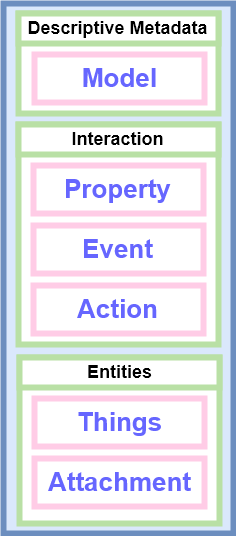
\includegraphics[width=4cm,height=8cm,keepaspectratio]{./Part2/Chapter6/figures/asset-descriptions-1.png}
	\caption{ : Overview Asset Model}
	\label{fig: Overview Asset Model}
\end{figure}
\subsection{Web of Things Framework}

Guinard \textit{et al.} propose a WoT framework that can generate a set of REST services to exploit and hierarchically link the sensor node resources via web interface\cite{guinard2009towards}. This speeds up creating ad-hoc applications for end-users. Their work is later applied in the AutoWoT project \cite{mayer2010facilitating} that aims to rapidly integrate IoT devices into WoT context by automatically building the web services to expose the device resources and functionality. AutoWot generates these web services based on a hierarchical service descriptions created by the end-user for the specific device. In addition, a graphical user interface is also proposed to facilitate creating description process for developers and tech-savvy users.\\

Another academic framework involving REST principle for integrating IoT devices into the Web is WebPlug \cite{ostermaier2010webplug}, a WoT framework including several functional blocks allows to represent and manage sensor data as the web resources. The users can compose their personal services based on physical objects. These services and resources accessibility is enhanced by Meta-URL that is proved to bring considerable benefits in temp of resource discovery and creating mash-up WoT applications. In the same approach, Christophe \textit{et al.} \cite{christophe2011web} proposes a framework for creating and handling IoT devices as virtual objects according to the event-based rule schema. The author in \cite{orestis2012towards} presents a service-oriented framework supporting multiple real-time services for  Wireless Sensor Networks (WSN) and smart objects via the Web such as storage, sharing, discovery. SemSense framework \cite{moraru2011exposing} aims to collect, process, equip with semantic meta-data and publish on the Web according the linked data standard. SPITFIRE \cite{pfisterer2011spitfire} targets to unlock the uni-modal closed systems in WoT by generating the semantic sensor description and an effective searching mechanism. After abstraction, the sensors and Things are integrated into Linked Open Data (LoD) cloud. This effort makes the collected data easily accessible on the Web and accelerates the development of WoT applications. With the convergence of academic and commercial worlds, several Web platforms are emerging with the aim to abstract the heterogeneity of the physical devices by REST web services. There are well-known framework such as Xively \cite{Doe:2009:Online}, ThingSpeak \cite{thinkspeak:Online}, and ThingWorx \cite{thingworx:Online}. These frameworks support accessing and visualizing the device data from cloud. Moreover, a RESTful API is offered for developer to build the custom application on the collected data.\\

In the light of this state-of-the-art, there are still missing the semantic description and a lightweight IoT architecture seamlessly presenting and managing the compound objects, which are monitored by multiple IoT devices.

\section{WoT Asset Description}
WoT Asset Description is considered as the major part enabling Web of Things in our propose. Before describing in detail, we have to identify the required components inside such Asset. The Asset must be able to briefly introduce and discovery itself via self-description meta-data. The existing resources and interaction method are also effectively described to be fully accessible via Web. In addition, the devices along with their services belonging to the Assess must be presented and managed via defined actions. 
% is composed of the self-description meta-data, resources, entities and services. In general, the meta-data section presents the general information of the Asset in Web context. The existing resources and interaction method are described in next section named Interaction. The last section named Entities consisting of the information attached things and service of the Asset.

Based on the structure and requirements outlined above, we propose the WoT Asses Description (WoT-AD), a semantic description considering as an abstract entry point of a group of Things enabling the effective discovering, accessing and management process. WoT-AD is an extended concept of the W3c Things description (W3C-TD), which uses a JSON-LD schema to describe the single Things. The WoT-AD structure consists of three primary sections as illustrated in Figure \ref{fig: Overview Asset Model}: 
(1) The Descriptive meta-data describes the general Asset information. 
(2) The interaction model presents the Asset Resources (ARs) under the semantic scheme.
(3) The Entities express the Things and services constituted of Asset and their relations. More details of each element are described below:
\begin{itemize}
	\item \textbf{Descriptive Meta-data Section:} This section characterizes the Asset by presenting the unique identifier (URI) along with general information such as name, model, description, link... 
	\item \textbf{Interaction Section:} This section presents the available resources and services on the Asset and the interaction method. Each resource is considered as an interaction pattern which contains two separated parts are descriptive meta-data and interaction information.  
	\begin{enumerate}
		\item Descriptive meta-data holds the general information and configuration of resources such as type, description.
		\item Interaction information holds the information to connect to the resources such as connection address, method.
	\end{enumerate}
	The interaction pattern is divided into three types: Property, Event and Action to present several resources. The Figure \ref{fig: Overview the WoT-AD interaction} illustrates the interaction section of a simple WoT-AD that uses to abstract a building floor as an Asset. 
	\begin{enumerate}
		\item The Property is used to express the state of Asset that is collected or calculated from the attached Things. The property value is timely updated by a mathematical formula complying with Virtual Sensor Framework. The end-user can directly access or observe such value via interaction information that is defined via URI. As shown in the example, the temperature of the meeting room in the floor is declared as an Asset property and updated from the average of environment temperature collecting by device 1 and device 2. An HTTP access API is also provided to obtain the value.
		\item The Event presents the special situation detected by a set of specific conditions on Property. When the condition is satisfied, the corresponding actions are triggered. For example, in Figure \ref{fig: Overview the WoT-AD interaction}, we identify the overheating event with the condition that the value of temperature property is higher than 30 degree and trigger the turn on air conditioner action. 
		\item The Action presents the supported functions of the Asset which could be triggered by the event. The user could also directly access and control the actuator via available services belonging the Asset. In the presented example, the turning on air conditioner action is trigger by the overheating event and the command is directly sent to actuator of device 3. 
	\end{enumerate}
	\item \textbf{Entities and Attachment Section:} This section describes the entities belonging to the Asset. In our proposal, the entity may be a Things or service named attachment. Each Thing contains the descriptive meta-data and the address to interact with Things resources and services. The attachment could be the cloud-based services such as open data server, repository, device management server. Such attachments are treated as a Things which has meta-data and interactive address.
\end{itemize}
\begin{figure}[h]
	\centering
	\frame{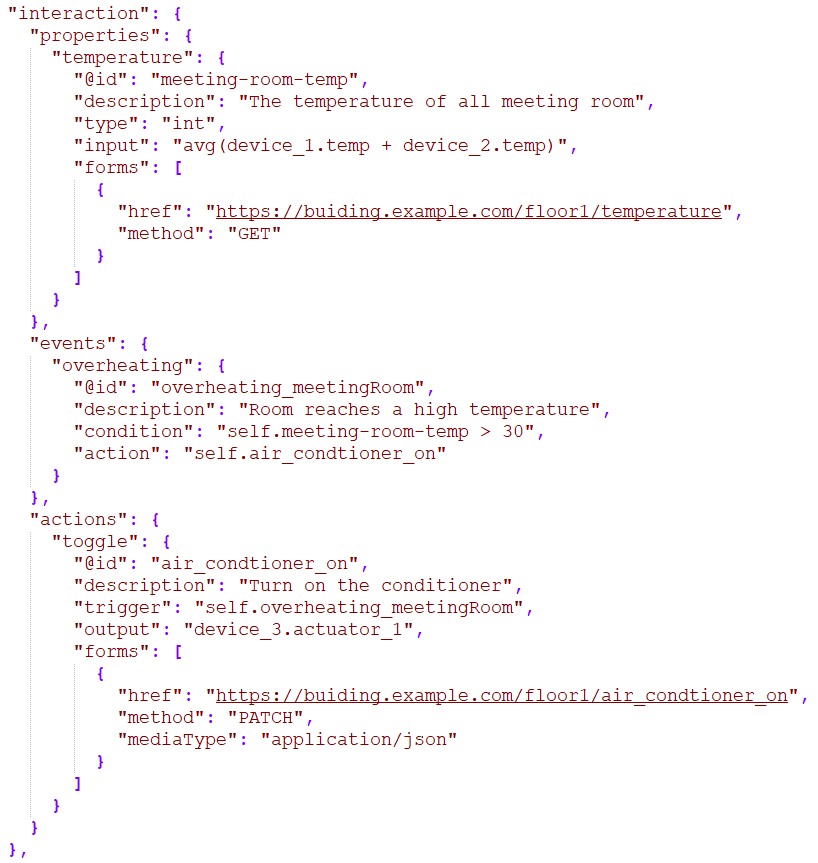
\includegraphics[width=0.9\textwidth]{./Part2/Chapter6/figures/wot-ad-2.PNG}}
	\caption{ : Overview the WoT-AD interaction section}
	\label{fig: Overview the WoT-AD interaction}
\end{figure}

\section{WoT Framework for WoT-AD}
\subsection{Principles and Design}
The overall goal of our proposal is to enable WoT for Asset in Massive IoT by providing a novel concept for Asset description along with an WoT framework. In addition, the framework facilitates the development of IoT applications on the Asset by providing a composition editor. For this reason, the designed architecture complies following principles:
\begin{itemize}
	\item High performance and low computational load for the server to adapt to Massive IoT scenario that must handle a large amount of connection.
	\item Effectively discovery, manage and access the Asset to fully aware of the real-world scenario. 
	\item Accelerating the development of IoT application on the Asset regardless of the user's skill.
	\item Handling the heterogeneity of constrained devices in LPWAN context. This enables the connection from a wide range of devices to framework effortlessly regardless of their characteristics. 
\end{itemize}
In order to archive these principles, we deal with several challenges listing below: 
\begin{itemize}
	\item The connectivity layer as the lowest part of architecture should be able to handle the connection from not only IoT devices but also the open data sources (open weather, open MQTT broker...). In addition, this layer needs to deal with the heterogeneity in term of LPWAN callback configurations. For example, the SIGFOX forwards the data via HTTP GET method whereas Lora Objenous uses HTTP POST method with different syntax. 
	\item The core of architecture must automatically discover and index the available resources in the Things which constitute of the Asset. These resources should be discovered in mash-up applications to facilitate the Asset creation procedure. This part also takes responsibility for real-time updating the Assess resources from collected data.
	\item The upper part of architecture must provide simple APIs to allow the user effectively discover, access and manage the Asset. A graphics editor is also provided to facilitate the Asset creation process.
\end{itemize}

\subsection{Overall Architecture}
\begin{figure}[h]
	\centering
	\frame{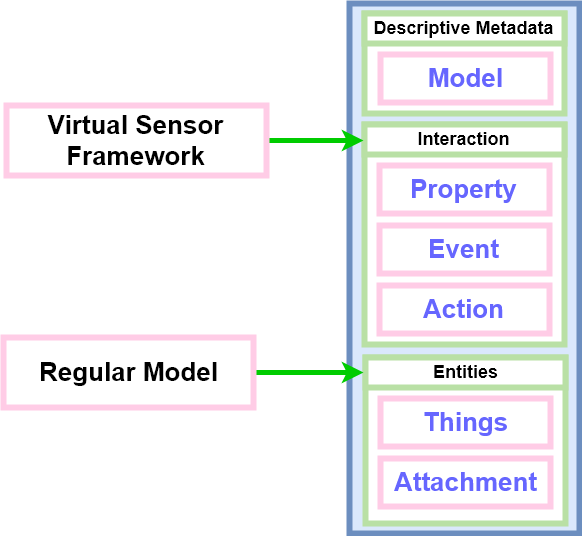
\includegraphics[width=8cm,height=12cm,keepaspectratio]{./Part2/Chapter6/figures/asset-operation-1.png}}
	\caption{ : Overview Operation Model}
	\label{fig: Overview Operation Model}
\end{figure}
Based on the listed principles and challenges, we propose a WoT framework fully exploit WoT-AD concept in Massive IoT scenario. The initial implementation of such architecture is represented by three main components spreading on horizontal layers, whose features properly fit the mentioned principles. The connector framework is used at lowest layer \cite{kim2017industrial} to handle the heterogeneous connections from both IoT devices and external data sources. The second component is the virtual sensor framework \cite{kim2017scalable}, an IoT framework supporting to create the logical data flow by visualizing the resources. The last component is a Graphic Editor facilitating the building and configuring process of the Asset by offering the drag-drop actions on HTML5 web interface. The overall of the framework is illustrated in Figure \ref{fig: Overview the Asset architecture}. The details of each layer are described below:
\begin{itemize}
	\item \textbf{Connection Layer:} This layer takes responsibility to handle the connection from LPWAN devices to the framework through dedicated connector. These connectors are simply created and managed by connector framework. At this layer, collected data from physical devices are aggregated and pre-process before conveying to upper layer. In case a new device connects to framework, the resources of this devices will be registered and tracked by sensor tracking services. 
	\item \textbf{Processing Layer} This layer is considered as a primary part of the architecture consisted of four main components: 
	(1) Virtual sensor platform is used to create the Asset by abstracting and linking the device resources together. This platform also has responsibility to update the Asset resources from collected data
	(2) Indexing: After successfully creating, the Asset resources are indexed by the indexing system. This guarantees all the resources are real-time discovered and synchronized with physical devices. 
	(3) Asset scripting is used to generate the Asset description and APIs based on defined resources. 
	(4) Asset model execution covert the Asset model to logical data flow \cite{kim2017scalable} be used by virtual sensor framework.
	\item \textbf{Presentation layer} This layer contains an interactive HTML 5 web interface, namely Asset Composer. This graphical interface provides the user several IoT components such as sensor, actuator, Asset, symbolic link. The end-user could simply create their own Asset by drag-drop actions. A dashboard to manage the existing Asset also proposed.
\end{itemize}

\begin{figure}[h]
	\centering
	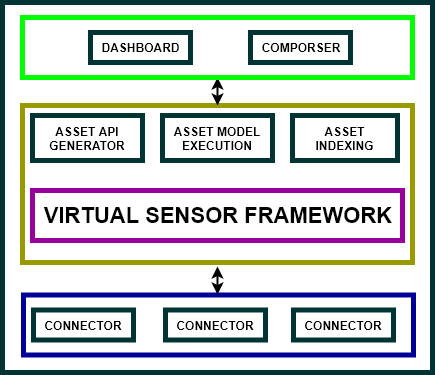
\includegraphics[width=0.65\textwidth]{./Part2/Chapter6/figures/overview_architecture.png}
	\caption{ : Overview the Asset architecture}
	\label{fig: Overview the Asset architecture}
\end{figure}

The primary requirement of WoT framework is that it must effectively and timely update and present the available resources. For this reason, we integrate our framework with a virtual sensor framework \cite{kim2017scalable} which provides self-discovery mechanism and supports generating the logical data flow from existing IoT devices. In general, an Asset is a self-operation object which is periodic updating its property values via an assigned logical data flow. The end-user can configure this frequency in Asset descriptive meta-data section.\\

The Asset's properties operate as a virtual sensor to retrieve and present the collected information from IoT sensors or devices. The elements in the Interaction section are build based on complex event processing (CEP) engine \cite{chen2014complex}. Therefore, if the current Asset properties reach a certain condition, the corresponding events are inferred and triggered the action. For example, we present the building floor as an Asset with the properties are the C02 and Humility of each room on the floor. If the CO2 degree of 75\% room is higher than 1000 ppm, the "suffocating" event is inferred and the system will send instruction command to relevant actuators to open window.


\section{Evaluation}
In order to validate the concept of WoT-AD and WoT architecture from the functional point of view, we have utilized the smart space scenario including a Raspberry Pi model B, which is considered as smart gateway be installed our WoT framework. In such context, the floors consisting of a set of rooms are considered as the Assets which are monitored by various IoT devices. Each device provides different resources and services. For example, the monitoring device equipped with multiple sensors including Co2, humility, PIR (motion detection), temperature, light. All collected information is used to control the air conditioning and light system for saving energy consumption. The control decisions are based on the whole floor status instead of the single room. Therefore, this context is the best practice to apply Asset. \\

Following the described scenario, a remote user can visually create and control an Asset via the interface of smart gateway. If the users use the existing Asset template, they only need to assign the IoT devices identification to the template. Based on this identification, these devices resources will be discovered and added to the interaction model of WoT-AD. Then, the complete WoT-AD is conveyed to processing layer where (1) Asset Script component creates the access API for the Asset resources, (2) Indexing component assigns a unique identity to the Asset for further self-discovery. Based on the composed Asset configure file, the logical-data flow is created to update the Asset properties from the collected information. This ensures the Asset data timely updated and reacted with the environment changes via configured events and actions in Asset's properties. \\

The software environment along with a light-weight local database for storing Asset configuration takes around to 100MB of spaces on the Raspberry Pi comparing with 32GB memory card. The most consumed operation of the framework is collecting, processing and updating the Asset information in processing layer. During the operational cycle mentioned in the scenario, the CPU load from 20 to 30 percent.
The high performance and scalability of such operation are ensured by Virtual Sensor Framework \cite{kim2017scalable}. 

\section{Conclusion}
In a nutshell, this work presents a semantic description for the physical Asset for enabling Web of Things in Massive IoT scenario. A WoT architecture is also defined and implemented to fully exploited the proposed concept. The architecture supports the interaction with various IoT devices and sensors based on the connector model implemented at lowest layer. The core element of the architecture is a framework named Virtual Sensor Framework that executes all the Logical data flow converted from Asset description. At the highest layer, we implemented a graphics editor fascinating the Asset description composing.\\
The effectiveness of designed solution was ensured by choosing and combining some technologies and IoT frameworks that have been practically demonstrated in real use-cases. To improve and extend the current works, we will optimize applied to smart building scenario. 

